% 完整编译: xelatex -> bibtex -> xelatex -> xelatex
\documentclass[UTF8,AutoFakeBold=1,AutoFakeSlant,zihao=-4]{cucthesis}

% 在这里填写你的论文题目
\newcommand{\thesisTitle}{《黑暗森林》游戏策划书}
\newcommand{\thesisTitleEN}{Game Design Document}

% 在这里填写你的相关信息
\newcommand{\yourDept}{计算机与网络空间安全学院}
\newcommand{\yourMajor}{游戏设计学}
\newcommand{\yourName}{王同学}
\newcommand{\yourClass}{2020级游戏策划01班}
\newcommand{\yourMentor}{王老师}
\newcommand{\studentID}{202020111222333}


\begin{document}

% 封面(自动生成)
\coverpage

% 中文摘要
\begin{abstract}
故事发生在一片虚构的大陆上。一股未知的力量袭击了这个世界,黑暗将一切吞噬,随之而来的是各种各样的怪物袭击,人类世界被摧毁殆尽。在希望即将破灭之际,终于人们发现这些怪物虽然强大,但是他们只能在黑暗中发挥出全力,在光明处虽然几率渺茫,人们还是有一战之力的。各地幸存下来的人们建立了数个巨型灯塔,并围绕灯塔建立了聚集地。为了维持这层光幕,这层人类最后的高墙,人们不得不深入黑暗的森林进行冒险。
\keywords{黑暗森林;游戏策划;角色扮演}     % 中文关键词
\end{abstract}

% 英文摘要
\begin{abstractEN}
The story takes place on a fictitious continent. An unknown force attacked this world, and darkness swallowed everything, followed by various monster attacks, and the human world was completely destroyed. At the time when hope was about to be shattered, people finally discovered that although these monsters are powerful, they can only exert their full strength in the dark. Although the chances are slim in the light, people still have the power to fight. The surviving people from various places built several giant lighthouses and built gathering places around the lighthouses. In order to maintain this light curtain, the last high wall of mankind, people have to go deep into the dark forest for adventure.
\keywordsEN{Dark Forest, Game Design, RPG}       % 英文关键词
\end{abstractEN}

% 目录(自动生成)
\contentpage

\section{游戏概述}

\subsection{游戏类型}
这是一款以模拟经营为辅的RogueLike游戏,它随机性与不可预测性强,适合重复游玩。

\subsection{游戏背景}
故事发生在一片虚构的大陆上。一股未知的力量袭击了这个世界,黑暗将一切吞噬,随之而来的是各种各样的怪物袭击,人类世界被摧毁殆尽。在希望即将破灭之际,终于人们发现这些怪物虽然强大,但是他们只能在黑暗中发挥出全力,在光明处虽然几率渺茫,人们还是有一战之力的。各地幸存下来的人们建立了数个巨型灯塔,并围绕灯塔建立了聚集地。为了维持这层光幕,这层人类最后的高墙,人们不得不深入黑暗的森林进行冒险。

\subsection{游戏特色}
游戏特色在于将模拟经营与探险融合起来,加入了Rogue Like元素。玩家不再是枯燥地等待自己经营的城镇发展或仅仅挑战预先设计好重复度高的探险。而是可以通过挑战不会重复的关卡去发展自己的城镇,通过发展城镇使得自己之后的挑战更有娱乐性。同时游戏内的“光亮系统”(玩家在探索时光亮会随着火把的消耗减弱,强大的敌人也会随时出现)在契合游戏背景的前提下为游戏添加了紧迫感,同时也能合理地限制玩家探索进度,延长游戏生命力。

游戏按照板块分类可以分为城镇部分、养成部分、地下城部分;而按照游戏人数分类可以分为单人部分以及联机部分,甚至可能有多人部分。


\subsection{游戏设计要点}
Rogue Like类游戏强调的是高随机性,而模拟经营则强调发展变强。要融合这两种游戏就必须平衡玩家发展变强的程度,否则游戏难度与乐趣到后期将大大降低。所以我们设计将游戏内招募到的人物职业技能数量限制在2-3个,符合职业特点的同时主要围绕着光亮与环境进行设计,实质伤害的技能减少,仅给玩家提供紧急的自保技能。


\section{游戏重要系统设定}

\begin{figure}[ht]
    \centering
    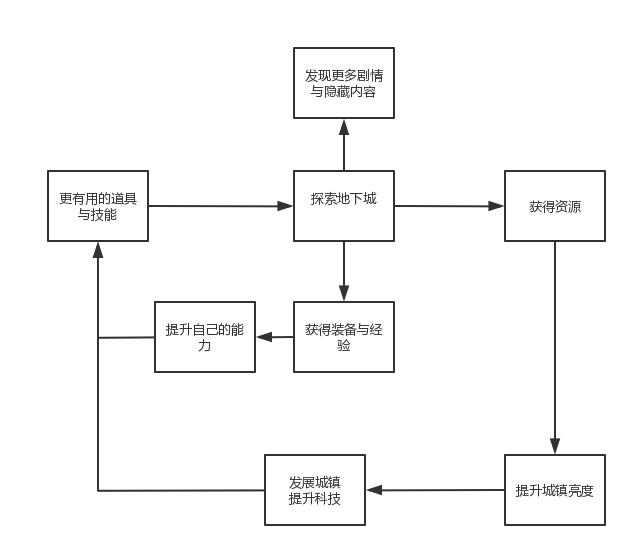
\includegraphics[scale=0.5]{imgs/游戏逻辑.png}
    \caption{游戏逻辑}
\end{figure}


\subsection{总体概述}
玩家拥有一个城镇作为自己的发展基地。但初始城镇功能有限,玩家需要通过不断的前往森林地下城探索资源来提升特定建筑的等级来获取更有用的道具和装备,为自己之后的冒险提供便利。

\textbf{城镇光亮系统:}
城镇中心有座灯塔,灯塔需要燃料来维持自己的照明范围。同时玩家可以提升灯塔等级或相关科技使灯塔扩大照明范围,但同样的,玩家需要更多的资源来维持其更大的照明范围。照明范围影响着建筑系统与森林地下城的难度。当其达到一定程度时可以解锁新的建筑与科技,同时玩家可以选择更深处的森林地下城进行探索。但需要注意的是,当燃料不足以维持灯塔亮度时,照明范围会缩小。带来的结果是照明范围外的建筑会重新被黑暗吞噬,甚至可能降低已经提升的建筑等级。

\subsection{探索系统概述}

\subsubsection{探索光亮系统}
玩家初次进入地下城时仅仅有3根火把(数量及照明设备可以通过提升城镇规模来进行升级),每根火把可以燃烧120秒,也就是2分钟。光亮也会在每个照明设备的3/3,2/3,1/3,0/3时分别进行“亮——>较亮——>微亮——>黑暗”的模糊渐变。根据亮度的变化会出现不同强度的敌人对玩家进行攻击,不同强度的敌人也会掉落不同强度的装备与资源。

\subsubsection{关卡系统}
玩家在进入森林地下城时,游戏会随机生成“种子”,并根据种子生成地下城以达到Rogue Like游戏的目的。我们并未采用一次性生成整张地图的游戏方式,而是采用了更为大众化的碎片式地图探索方式进行游戏。每一层都有一个BOSS镇守,玩家需要打败BOSS才能进入下一层地图进行探索。

\begin{figure}[ht]
    \centering
    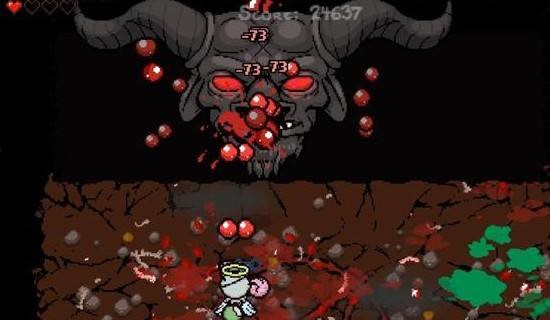
\includegraphics[scale=0.72]{imgs/《以撒的结合》BOSS战.jpg}
    \caption{《以撒的结合》中惊险刺激的BOSS战}
\end{figure}


同时关卡中会随机生成补给点与商店等,供玩家进行短暂的休整以降低游戏的难度,玩家可以在补给点或者商店重新点亮火把或是购买火把进行重整。每一层的初始点与BOSS点都设有“火焰传送门”,玩家可以通过传送门返回城镇来结束本次冒险。但要注意,通过初始点的传送门进行离开时会给予玩家包括资源折半,愧疚debuff等一定惩罚。


\subsubsection{随机事件}

在探索的过程中会出现随机事件,可能是更强大的敌人出现,也可能遇到其他冒险者的尸体,可能遇到重要NPC,甚至是进入了一个失落的遗迹等,为游戏添加更多的探索性。

\begin{figure}[ht]
    \centering
    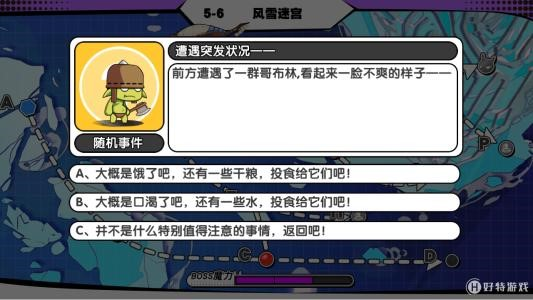
\includegraphics[scale=0.64]{imgs/突发事件.jpg}
    \caption{游戏中的突发事件}
\end{figure}


\subsection{战斗系统}

本游戏采用的是即时战斗系统而非回合制系统。我们认为回合制战斗系统不能将本游戏光亮系统的压迫感完美地体现出来。即时战斗系统允许玩家进行躲避,移动攻击,利用地形等操作,玩家可以通过职业特有的攻击方式对怪物进行攻击(战士盗贼类职业近战攻击,射手法师类则为远程攻击)。这种攻击方式常见于各类RPG游戏。


\subsection{伤害系统}

\subsubsection{伤害判定与击退效果}

本游戏采用碰撞的方式进行伤害判定,玩家被怪物攻击到或是碰撞到特定怪物会进行伤害计算,并可能伴随击退效果。同时会在游戏中的血条槽进行显示,并提醒玩家受到伤害。例如:玩家人物触碰到“骷髅法师”释放的冲击波或是碰到具有近身伤害效果如带有“收割灵魂”护体的“缚灵者”将会受到伤害,但后者并不会触发击退效果。或碰到了当玩家血条槽为空时则会死亡,同时当玩家濒临死亡时游戏周围画面会变红以提醒玩家注意血量。

\subsubsection{怪物死亡}
怪物死亡时会触发死亡动画,但详细的死亡效果将会按照普通怪物、特殊怪物进行分类。普通怪物播放完死亡动画后会掉落物品,尸体会缓慢消失;特殊类怪物播放完死亡动画后也会掉落物品,但尸体不会消失。

\subsubsection{玩家死亡}
玩家死亡后,屏幕会逐渐变暗,BGM也会有相应变化。屏幕暗到一定程度时弹出“返回城镇”按钮。玩家点击后将会返回城镇,此人物视为“失踪”状态。同时本次探险中玩家所有资源都将会丢失,并视为经过了一次冒险机会,即“过了一天”。此人物可能会出现在后续的救援任务中或直接以“事件”的形式出现在之后的探险中。


\subsection{操作系统}
玩家可以通过移动,躲在掩体后来躲避敌人的攻击。而每个职业拥有自身独特的躲避方式,例如战士可以举起盾牌来减免特定方向的攻击,法师可以通过短距离闪现来躲避敌人攻击,而射手可以通过快速翻滚进行躲避。

本游戏操作采用的是手机上“摇杆”类操作方式,即一只手通过触屏滑动控制人物移动方向,另一只手操作人物释放技能。
如图\ref{fig:stick01},\ref{fig:stick02}所示。

\begin{figure}[ht]
    \centering
    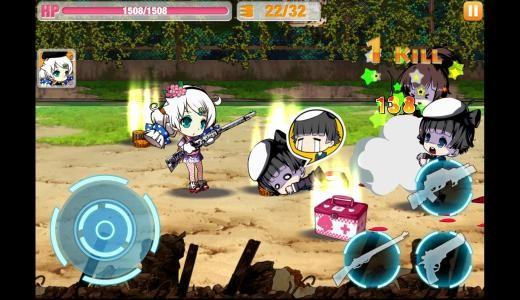
\includegraphics[scale=0.64]{imgs/崩坏2摇杆.jpg}    
    \caption{崩坏学园2中的“摇杆”操作方式}
    \label{fig:stick01}
\end{figure}


\begin{figure}[ht]
    \centering  
    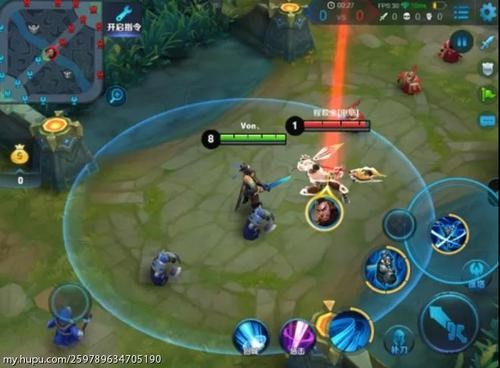
\includegraphics[scale=0.64]{imgs/王者荣耀摇杆.jpg}
    \caption{王者荣耀中的“摇杆”操作}
    \label{fig:stick02}
\end{figure}

这种“摇杆”类操作方式已经普遍运用到各类手机游戏中去,并没有技术上的难点。



\subsection{养成系统}

\subsubsection{人物养成}
玩家操作的人物通过招募而来。人物按职业来进行分类,除了个别“英雄”单位外,其他同职业人物并没有太大的显著区别。人物的培养可以分为技能、装备、变异特性的培养。

\begin{itemize}
    \item 技能:
    技能的采取“天赋树”的形式进行升级。当人物升到一定等级时可以进行“多选一”的技能选取。
    \item 装备:
    人物装备的获取采取地下城掉落以及完成任务以及商店购买的方式获取。地下城特殊装备仅能在每层“宝箱房”内拾取获得,并且不能被带出地下城。通常这些特殊装备要更为强力,这也是为了突出随机带来的乐趣。
    \item 变异与特性:
    人物在一定亮度以下或在特殊事件中会受到黑暗侵蚀,有几率获得特殊的变异。这些变异可能会对玩家带来有利或不利或好坏参半的特性,这些特性会予以保留,但在数量上会有最大上限。如何获取心仪特性以及各种特性之间会产生怎样的“化学反应”都将是玩家培养的乐趣所在。
\end{itemize}



\subsubsection{非人物养成}


\textbf{怪物捕捉:}有些种类的怪物是可以被捕捉驯化的。随着玩家在地下城中探索的深入,玩家会遇到越来越强里的怪物。玩家科技的提升能提升怪物的捕捉几率。捕捉到的怪物按种类可以分为守卫类以及支援类。守卫类如守护巨龙,可以作为坐镇BOSS帮助玩家守护自己的宝库或在工会战中作为BOSS出现抵挡其他公会入侵。支援类则可以在玩家探险中进行支援。这种方法可以为“非人民币玩家”提升游戏参与感,他们为工会捕捉到强力怪物也能得到其他人的赏识,让他们觉得自己也是工会中的重要一员,并不仅仅是“人民币玩家”的陪玩。

\textbf{城镇:}城镇的拓展首先建立在核心建筑“灯塔”的光量范围上。建筑必须建在灯塔照亮的范围内,否则不能建造。灯塔照亮的范围随着提供的燃料数量的增加而增加。而对灯塔这一建筑的提升可以提升灯塔对燃料燃烧的上限,即提高最大照亮范围。如果燃料不足以维持灯塔当前光亮,照亮范围将会减少,一些地区将会重新被黑暗吞噬。如果这些被重新吞噬的地区上有建筑的话,建筑将会被视为摧毁,需要重建。

\textbf{建筑系统:}城镇中有道具商店,锻造商店,任务告示栏,科技研究所,仓库,灯塔,酒馆,祭坛等场所。可以进行升级。


\begin{itemize}
    \item 灯塔
    负责城镇的照明范围,当燃料耗尽时会以最低亮度进行照明。
    科技提升:提高燃料转换效率,提升照明时间。
    建筑提升:提高照明最大范围。
    \item 道具商店
    为玩家提供冒险道具,包括火把,燃烧瓶等战斗中道具。
    科技提升:为玩家提供更多种类的探险补给品。
    建筑提升:道具一次性存货更多,降低道具售价。
    \item 锻造商店
    允许玩家分解装备,融合材料,打造装备。
    科技提升:允许玩家分解融合更高级装备,同时提供多基础装备打造配方。
    建筑提升:打造融合分解等操作消耗时间更少,收取费用更低。高等级时支持多装备同时操作。
    \item 任务告示栏
    为玩家提供各式各样的探索任务,同时提供相应的奖励。
    科技提升:会出现更高难度的任务。
    建筑提升:刷新的任务最大数量提升。
    \item 科技研究所
    允许玩家提升建筑与自身相应科技。
    \item 仓库
    允许玩家将资源装备等存入。
    科技提升:允许存放特殊物品。(如漆黑之石等)
    建筑提升:提升物品存放的最大重量。
    \item 酒馆
    随机刷新各种人物,触发某些事件后有几率刷新出稀有人物。玩家可以招募这些人物。同时有几率会有神秘商人出现在酒馆。
    科技提升:稀有人物出现几率提升,神秘商人出现几率提升。
    建筑提升:出现的人物最大数量提升,招募消耗变低。
    \item 祭坛
    通过祭献特殊物品可以使下一次森林地下城变为特殊的地下城。
\end{itemize}

\textbf{科技系统:}随着城镇的升级,玩家可以进行科技上的升级。这些升级会对玩家接下来的探险提供各种各样的帮助。比如:燃烧时间更长的油灯,更加强力的药剂以及更容易与其他城市进行贸易来获取需要的物资。


\section{联机部分}
联机部分提供了PVP模式以及合作模式。PVP模式包括宝库入侵。合作模式包含了拯救以及永恒之塔两种。

\subsection{PVP模式}
\subsubsection{宝库入侵}
每个玩家的城镇中都有宝库,玩家可以花费材料进行防守布局,同时支持玩家捕获特定的地下城怪物来帮助自己镇守包库。入侵的玩家在入侵宝库时会有一个时间限制,如果玩家在规定的时间内击败了防守方的BOSS并打开了宝箱,则视为入侵成功,可以得到被入侵方一定材料并可能获得宝物。如果时间结束或者死亡,则视为入侵失败,防守方可以得到防守奖励。
\subsubsection{工会战}
与宝库入侵相似,每个工会都会有一个工会宝库。工会宝库的大小会随着工会等级进行提升。每半个月进行一次工会战。一次有2-3个工会进行混战。每个工会的玩家每天都可有数次机会对交战公会进行入侵,成功入侵则会获得相应分数。最终按排名予以奖励。


\subsection{合作模式}
\subsubsection{拯救}
拯救模式救援:RogueLike游戏可分为完全随机以及伪随机生成方式两类。本游戏采用的是后者生成方式,即按照随机生成的生成码生成地下城场景。
如图\ref{fig:code}所示。

\begin{figure}[ht]
    \centering
    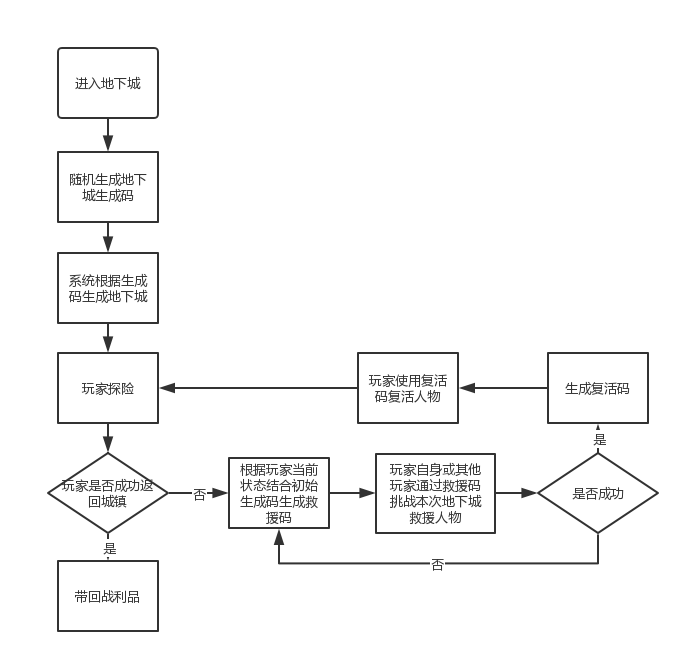
\includegraphics[scale=0.64]{imgs/生成码.png}    
    \caption{“生成码”工作流程图}
    \label{fig:code}
\end{figure}

\subsubsection{永恒之塔}
玩家从底层一层一层往高层进发,玩家爬的层数越高,获得的奖励越多。永恒之塔模式能将玩家装备威力发挥到最大,也是玩家强大实力的最好证明。同时会有层数排行榜,供玩家进行竞争。


\section{角色与技能设定}
游戏将为玩家提供4种选择角色职业,四个职业的背景故事发生在虚拟魔幻世界中一块独立的魔幻大陆,几百年前,大陆曾是一个统一的国家,由于国王的三个儿子都想继承王位,导致国家发生内战,为了平息战乱并获得王位,大王子利用黑暗的力量统一了整个大陆,战乱虽然平息,但是隐藏的危机却源源不段, 仿佛黑暗中一股强大的虎视眈眈的想随时吞噬整个大陆。几百年过去了,可怕的事情终于发生,大陆各处都发生了怪物吞噬民众的怪事,而且部分区域已经发生了大面积的骚乱,叛乱者居然是来自黑暗世界的魔物,为了维护大陆的和平,国王招募了一批优秀的年轻的勇士来想黑暗势力进行讨伐。比如:战士,具有更强的生命力和体力,善于战斗,属于力量型的角色,能使用绝大部分的武器与道具,能装备盔甲等重型防御装备,然而他的魔法防御很低;还有巫师,能使用魔法性的道具和武器,只能装备法袍等装备,因此魔法防御高,魔法攻击力强,但物理防御力很低,容易受到物理伤害;还有射手,属于敏捷型角色,闪躲能力高,不容易被敌人击中,而且攻击速度快,各项能力都比较均衡;还有刺客,刺杀型角色,使用精湛的刺杀技巧,但血量中等。于是,国王招募了一批优秀的年轻的勇士以后,他们为国家讨伐黑暗势力的战争就开始了。

\subsection{战士}

\begin{figure}[ht]
    \centering
    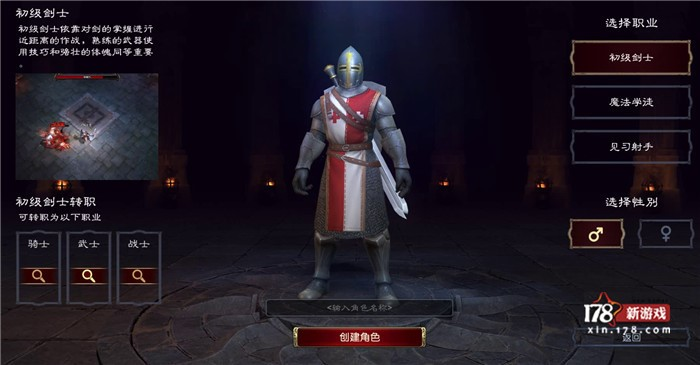
\includegraphics[scale=0.5]{imgs/战士.jpg}    
    \caption{战士职业示意图}
\end{figure}

特性介绍:力量型的角色,能使用绝大部分的武器与道具,能装备盔甲等重型防御装备。
优点:攻击力高,HP值高。缺点:移动速度低,机动性差。
上手难度:$\star\star$

\begin{itemize}
    \item 举起盾牌:朝玩家指向方向举起巨大的盾牌,可以减免来自盾牌方向的所有攻击。
    \begin{itemize}
        \item CD:6s/5s/4s/3s/2s
        \item 伤害减免:60\%/65\%/70\%/75\%/80\%
        \item 备注:本技能无法阻挡非线性攻击,例如:地火(在地方脚下召唤法阵,延迟后喷出火焰来攻击玩家)
    \end{itemize}

    \item 狂风斩:全力挥动武器对前方的怪物进行旋转连斩攻击,对战士周围的怪物造成伤害。
    \begin{itemize}
        \item 冷却时间:20s/18s/16s/14s/12s
        \item 持续时间:3s/4s/5s/5s/5s
        \item 备注:玩家释放本技能时可以将非BOSS的远程攻击击落,玩家释放技能时无法终止技能。
    \end{itemize}
\end{itemize}


\subsection{法师}

\begin{figure}[ht]
    \centering
    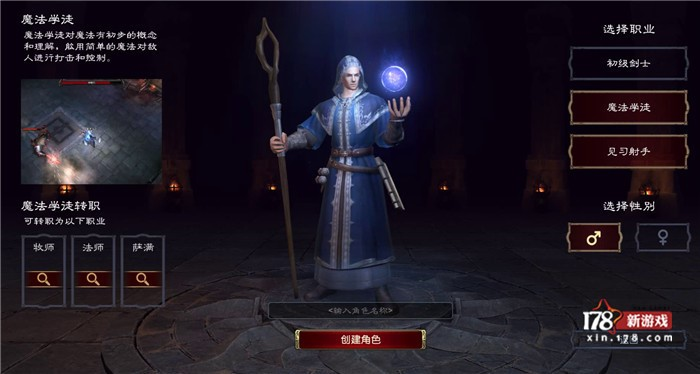
\includegraphics[scale=0.5]{imgs/法师.jpg}    
    \caption{法师职业示意图}
\end{figure}

特性介绍:智力型角色,能使用魔法性的道具和武器,只能装备法袍等装备。
优点:魔法防御高,魔法攻击力强。 缺点:物理防御力很低,容易受到致命伤害。
上手难度:$\star\star\star\star$


\begin{itemize}
    \item 闪烁:朝玩家指向方向进行短距离传送来规避敌人的攻击。
    \begin{itemize}
        \item CD:10s/9s/8s/7s/6s
        \item 闪烁距离:1码/1.5码/2码/2.5码/3码
        \item 备注:本技能允许玩家进行跨越地形的操作。
    \end{itemize}

    \item 魔法飞弹:向怪物发射魔法飞弹,共持续3秒,对飞弹触碰到的目标造成伤害。
    \begin{itemize}
        \item CD:8s/8s/8s/7s/7s
        \item 每秒发射个数:1个/2个/2个/2个/3个
        \item 备注:技能释放期间玩家无法移动。但是玩家可以通过移动或闪烁来强制打断技能。
    \end{itemize}
\end{itemize}


\subsection{射手}
\begin{figure}[ht]
    \centering
    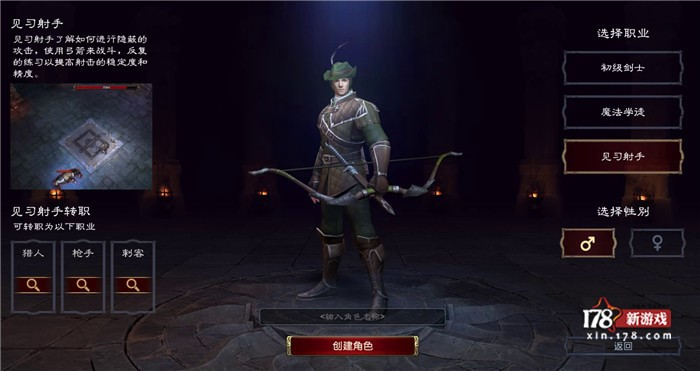
\includegraphics[scale=0.5]{imgs/射手.jpg}    
    \caption{射手职业示意图}
\end{figure}

特性介绍:敏捷型角色,使用远距离攻击武器。可以装备部分重型防御装备。 
优点:闪躲能力高,不容易被敌人击中,而且攻击速度快。缺点:无法应对近距离敌人 。
上手难度:$\star\star\star$

\begin{itemize}
    \item 翻滚:朝玩家指向方向进行中距离翻滚以规避敌人的攻击。
    \begin{itemize}
        \item CD:10s/9s/8s/7s/6s
        \item 翻滚距离:2码/2.5码/3码/3.5码/4码
        \item 备注:本技能不允许玩家进行跨越地形的操作。
    \end{itemize}

    \item 风暴射击:以风暴之势迅速向玩家指定方向射出数支强有力的箭矢,对接触到的敌人造成伤害。
    \begin{itemize}
        \item 冷却时间:15s/13s/11s/10s/10s
        \item 箭矢数量:3支/4支/5支/5支/6支
        \item 备注:释放本技能时不能转向,不能释放其他技能。
    \end{itemize}
\end{itemize}


\subsection{刺客}
\begin{figure}[ht]
    \centering
    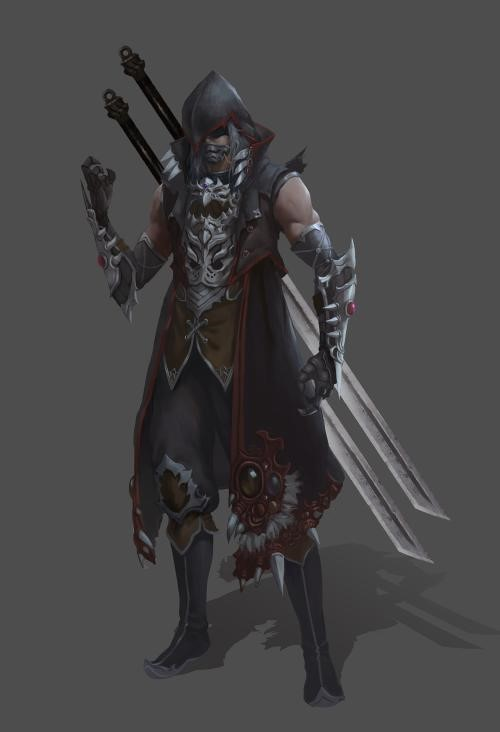
\includegraphics[scale=0.24]{imgs/刺客.jpg}    
    \caption{刺客职业示意图}
\end{figure}

特性介绍:收割型角色,有着很强单体杀伤力的角色,他们往往有着秒杀单个怪物的能力,但是自身却比较脆弱。
优点:速度快,伤害高;缺点:血量少,对群体敌人应对手段少。
上手难度:$\star\star\star\star\star$

\begin{itemize}
    \item 招架:瞬间进入规避状态,完全招架敌人的攻击。
    \begin{itemize}
        \item CD:6s/5s/4s/3s/2s
        \item 持续时间:0.2s/0.3s/0.4s/0.5s
        \item 备注:本技能效果持续期间进入无敌状态,无视一切攻击。
    \end{itemize}

    \item 潜行:进入潜行状态,不会被敌人发现。
    \begin{itemize}
        \item CD:20s/20s/20s/20s/20s
        \item 持续时间:5s/6s/7s/8s/10s
        \item 备注:使用道具或释放技能或攻击会打破潜行。
    \end{itemize}

    \item 生命收割:瞬间移动到目标身后,如果敌人生命值低于一定比例,则对敌人造成巨额伤害,否则造成普通伤害。如果敌人死于生命收割,则CD减半。
    \begin{itemize}
        \item CD:12s/12s/12s/10s/10s
        \item 血量比例:10\%/15\%/20\%/25\%/30\%
        \item 备注:无。
    \end{itemize}
\end{itemize}


\subsection{BOSS举例}
\begin{figure}[ht]
    \centering
    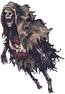
\includegraphics[scale=1.0]{imgs/极恶骷髅.jpg}    
    \caption{极恶骷髅示意图}
\end{figure}

说明:由黑暗创造并且生活于地牢的一种怪物,攻击方式多样,使用武器骨刺,拥有敏捷的速度和强大的力量。
动作:攻击,被攻击

\begin{itemize}
    \item 听我号令:极恶骷髅会在自身周围召唤1-2只骷髅战士和1-2只骷髅弓箭手帮助极恶骷髅攻击玩家。
    \item 光明收割:极恶骷髅会瞬移到屏幕中央进行短暂读条,读条结束后会将玩家的光亮值瞬间将为0,进入黑暗状态。
\end{itemize}


\subsection{普通怪物举例}

\begin{figure}[ht]
    \centering
    
\includegraphics[scale=1.0]{imgs/史莱姆.png}    
    \caption{史莱姆示意图}
\end{figure}

说明:一种软体动物,具有一定的魔力,通过大地的灵气而产生的生物。
动作:攻击,被攻击。粘液喷射:朝玩家方向喷射短距离粘液,被喷射到的玩家会暂时降低速度。


\section{美术与音效}

\begin{figure}[ht]
    \centering
    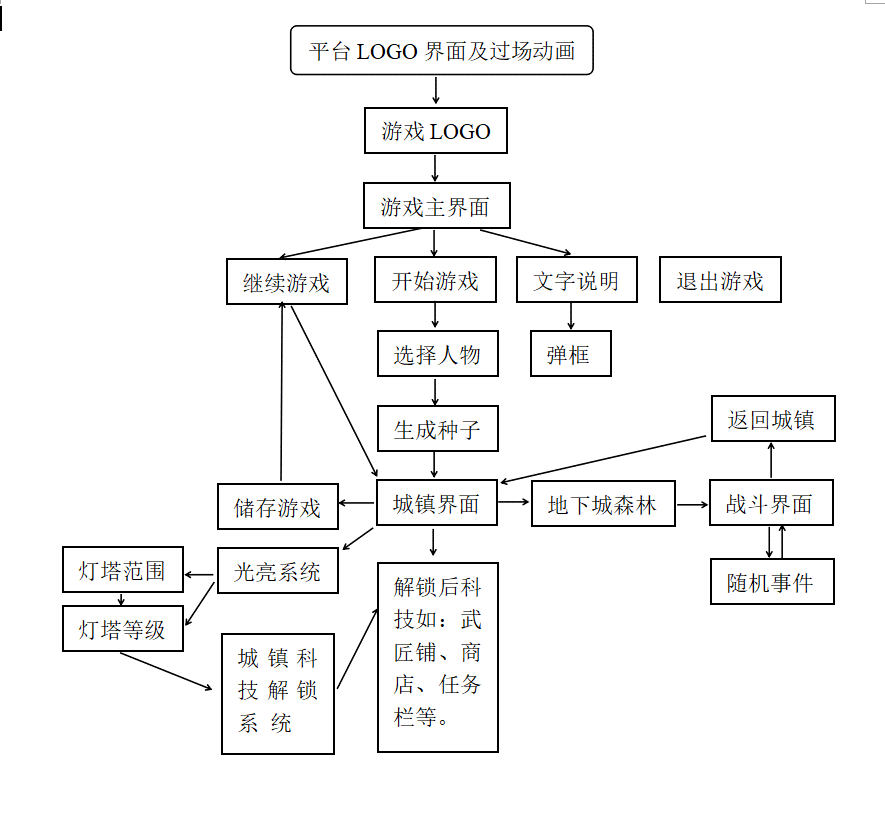
\includegraphics[scale=0.5]{imgs/界面流程图.png}    
    \caption{游戏界面逻辑流程图}
\end{figure}

\subsection{游戏开始界面}

游戏开始界面左下侧出现:新游戏,继续游戏(进入新游戏储存后出现),游戏文字说明,退出游戏选项。游戏背景为中世纪古堡图片。

\begin{figure}[ht]
    \centering
    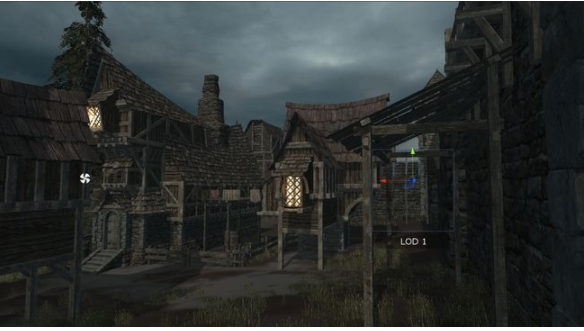
\includegraphics[scale=0.8]{imgs/游戏背景.png}    
    \caption{游戏背景示意图}
\end{figure}

\subsection{人物选择界面}

界面中可见提供玩家选择的1个角色,和锁定角色(由第一个角色经过一系列完成任务后可解锁),红色选择框选择到一个角色时,左上方出现角色说明,背景出现角色图像,三个角色的选择框在下方。选择好后点击下方开始选项。

\begin{figure}[ht]
    \centering
    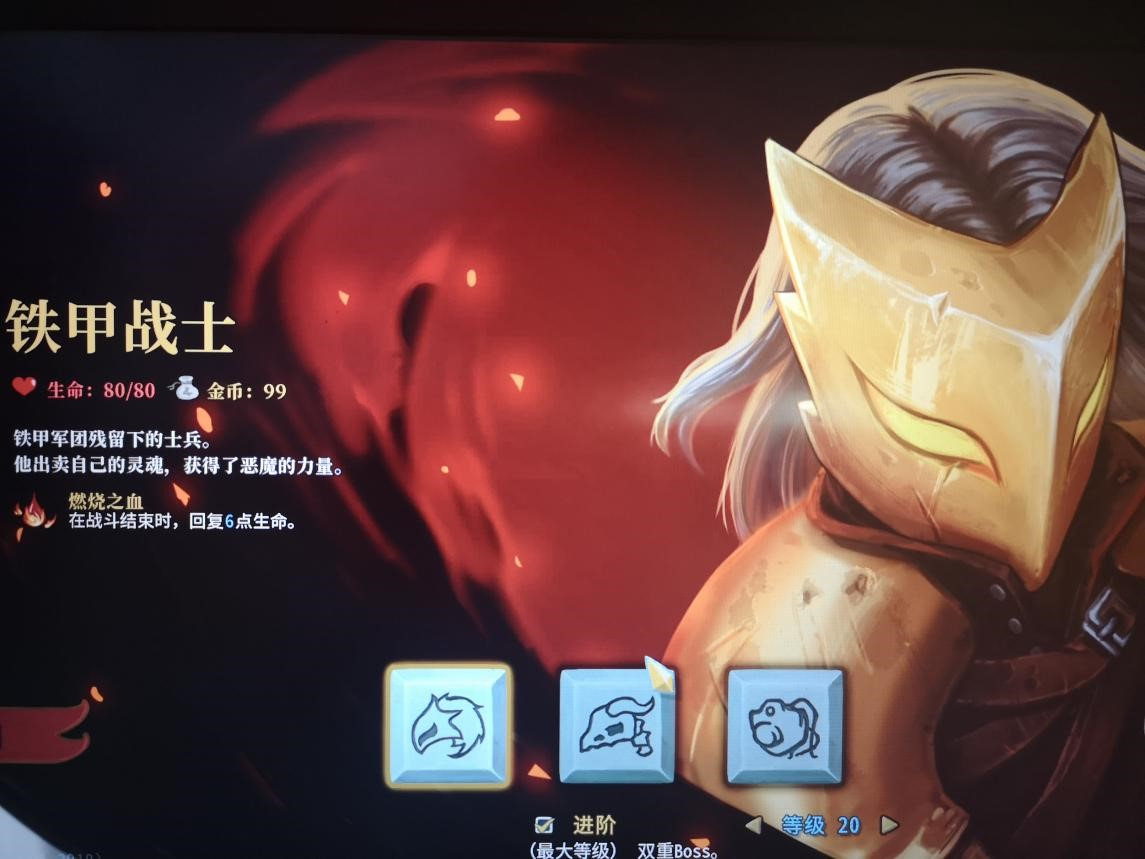
\includegraphics[scale=0.64]{imgs/角色选取.jpg}    
    \caption{角色选取界面概念图}
\end{figure}

\subsection{战斗界面}

\begin{itemize}
    \item 生命槽:
    生命槽是界面左上方显示人物所能承受伤害的横条,对应人物的生命值。在森林中与怪物搏斗未能躲避或防御时,将缩短生命槽,当使用回复生命的物品时,生命值将会增加。生命槽满时,人物可以承受100点伤害,当被怪物攻击到生命值空时,人物死亡,游戏结束,画面将被黑暗笼罩,黑暗中将出现重新开始和退出游戏选项。
    \item 火把倒记时:
    为了体现游戏黑暗主题和玩家的刺激感,还有玩家更方便的计算火把时间从而选择继续探险还是打道回府。屏幕最中上方将出现火把倒计时,每一个火把时间为120秒,当80秒的时候,随着时间减少,画面将逐渐由四周到中心越来越黑暗,当玩家重新使用新火把时,时间重新变为120秒。当火把时间到达0时,画面将仅显示人物周边及小范围,其他地方尽是黑暗。
    \item 护甲槽:
    除了生命槽外,还有一条特有的护甲槽。护甲槽位于生命槽下方,当收到怪物伤害时,将优先扣除护甲槽值,当护甲扣光后,再进行缩短生命值,在游戏中,可花金币修复装备,(类同于修复装备耐久)护甲值将增加。
    \item 人物:
    人物的每一个动作都有不同的姿势,如拾取、战斗、打开、合成装备等。玩家可以通过界面中的人物动作来判断其使用的技能和所处的状态。
    \item 聊天室:
    聊天室是界面左下角一条文字框,类似于魔兽世界聊天系统,点击后将打开成矩形,可以看见其他人的对话内容。
    \item 物品槽:
    在界面下方将有一长矩形,在矩形中分割为数个小方块,每个小方块可以放一个物品,物品右下角将显示数字,为物品的数量。使用鼠标可拖动物品到另一个方块中。
    \item 城镇:
    城镇是游戏中的另一个界面,界面主要是中世纪建筑图像,在界面左侧有4个选项,休息:玩家回复满生命值,修建燃料所:增加城镇的光照范围以解锁城镇更多的地方,武匠铺:点击后界面右方将出现装备框(类似于暗黑破坏神2),可以进行升级、合成、修理,储存:储存游戏。    
    \item 解锁功能:
    在玩家解锁越来越多的光照范围,将恢复其地区功能,如高级材料店、高级恢复店等。每解锁一个后将在城镇界面左侧选项中增添如“高级材料店”的选项。
    \item 战斗画面风格:
    游戏采用偏向于哥特式,色调偏暗的2D美术风格,用黑暗带给用户压迫感和紧张感,战斗时人物会有挥舞动作,并在怪物头顶会出现造成的伤害,怪物追击人物时会有特殊音效。    
\end{itemize}

\begin{figure}[ht]
    \centering
    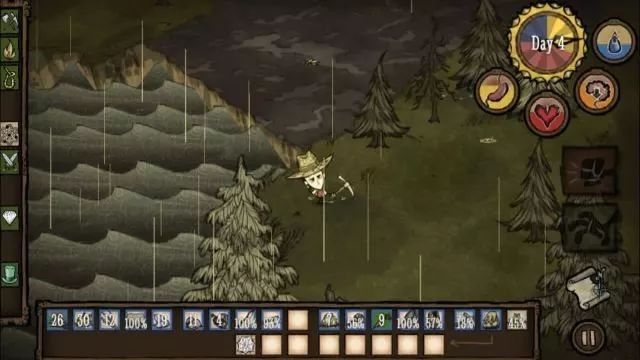
\includegraphics[scale=0.5]{imgs/游戏概念图.jpg}    
    \caption{游戏概念图}
\end{figure}

\subsection{美术风格}
鉴于要展现的是一个黑暗的魔幻世界,本游戏采用偏向于哥特式,色调偏暗的2D美术风格。而建筑则为偏向于中世纪欧洲的建筑风格。
哥特式风格偏向暗系,可以将玩家在森林中的黑暗无所不在的压迫感表现得淋漓尽致,能使得玩家在重见光明时的欣喜提升到最大。类似于盐和庇护所和地下城堡2等游戏。

\begin{figure}[ht]
    \centering
    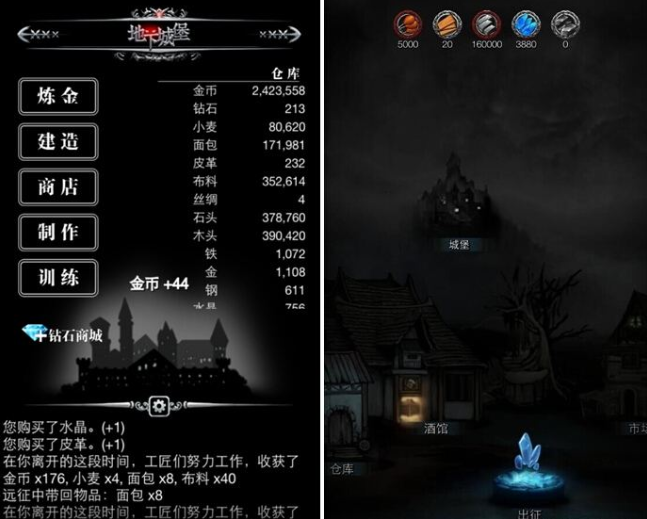
\includegraphics[scale=0.8]{imgs/美术风格01.png}    
    \caption{《地下城堡》偏向黑暗色系的风格}
\end{figure}

\begin{figure}[ht]
    \centering
    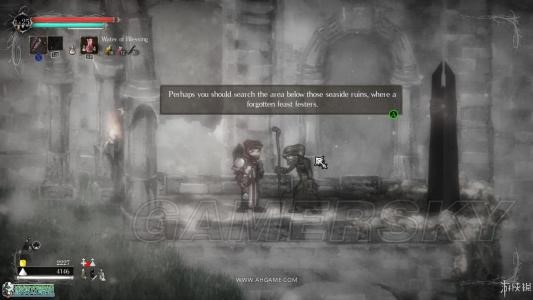
\includegraphics[scale=1.0]{imgs/美术风格02.jpg}    
    \caption{《盐和避难所》给玩家朦胧感的艺术风格}
\end{figure}

但是本游戏在光照上将更加黑暗,人物更加精致。建筑风格与环境的搭建将参考中世纪欧洲建筑风格。玩家在探索中也会见到各种失落的中世纪欧洲城市与遗迹,更加符合玩家审美。


\section{盈利模式}
本游戏可采取微买断+内部道具收费的方式进行盈利。玩家仅需十几元或几元即可游玩游戏。以低价格高质量吸引有消费潜力的玩家。而收费道具则可有建筑加速、强力卷轴,永恒之塔的复活以及入侵时的血瓶等。玩家爬塔爬到高层时死亡一定会对复活特别渴望;玩家入侵包库即将成功时一定不会吝啬对血瓶的使用,这些玩家非常重要但不是必需的内容都是可以进行内部收费的道具。

\section{竞品分析}
市面上RogueLike类的地牢探险主要集中在独立单机游戏中,主要的竞争目标为“元气骑士”。元气骑士进入市场较早,用户基础好,但本人认为它的制作较为简单且粗糙,并且其养成部分是些无关痛痒的养成,例如家园装修,并没有将养成和探险有效结合起来。并且他的联机部分仅有合作探险,并没有好的PVP部分,玩家没有有效途径炫耀自己的努力成果,社交性极差。而本游戏的PVP以及救援模式则提供了这种功能,玩家突破了其他玩家的防御,或好朋友、异性朋友向自己求助而自己完成了救助,这种自豪感可以有效促使玩家继续游玩甚至是充值购买道具。同时本游戏也在如何提升低消费玩家游戏参与度上提出了解决方法。玩家在游戏的重要一环——怪物捕捉与工会战中可以发挥自己的作用。非高消费的游戏热爱者可以在更困难的地下城中凭借自己的游戏技巧为公会捕捉到强力怪物,使自己的怪物成为工会在工会战中的“中流砥柱”,提升玩家的参与度与自豪感,这是很多游戏没有考虑到的。保持住了非高消费玩家的用户量,自然会有高消费玩家加入并进行消费。


% 参考文献(自动生成)
\begin{references}
    \bibliography{references.bib}
\end{references}

\nonumsection{附录}
\appendixformat     % 作为附录时,使用该命令为图表更新格式
无\cite{bib01}

\nonumsection{后记}
无\cite{bib02}

\end{document}
